% showcase.tex -- standalone presentation of the semi-structures package
% Build from this directory with: pdflatex showcase.tex (twice)
\documentclass[11pt]{article}

\usepackage[letterpaper,margin=0.72in]{geometry}
\usepackage{graphicx}
\usepackage{booktabs}
\usepackage{array}
\usepackage{float}
\usepackage{xcolor}
\usepackage[font=small,labelfont=bf]{caption}
\captionsetup{justification=raggedright,singlelinecheck=false}
\usepackage{tikz}
\usetikzlibrary{arrows.meta,positioning}
\usepackage[hidelinks]{hyperref}
\hypersetup{
  pdftitle={semi-structures Python Package},
  pdfauthor={Matthew Wormington},
  pdfsubject={Material-aware 2D diagrams, process-flow models and true 3D solids}
}

\graphicspath{{figures/}}
\setlength{\parindent}{0pt}
\setlength{\parskip}{0.55em}
\setlength{\tabcolsep}{5pt}
\renewcommand{\arraystretch}{1.18}

\definecolor{slate}{HTML}{3D4852}
\definecolor{lineblue}{HTML}{255C99}
\definecolor{softblue}{HTML}{ADD8E6}
\definecolor{softsand}{HTML}{F2EAD8}
\definecolor{softgold}{HTML}{E5C766}
\definecolor{palegray}{HTML}{ECEEF1}

\newcommand{\packagefile}[1]{\texttt{#1}}
\newcommand{\capability}[1]{\textcolor{lineblue}{\textbf{#1}}}
\newcommand{\generatedwith}[1]{(Generated with \packagefile{#1})}
\newcommand{\kinddsl}{\textcolor{lineblue}{\textbf{Process DSL.}}\ }
\newcommand{\kindspecial}{\textcolor{slate}{\textbf{Special purpose.}}\ }

\begin{document}
\pagenumbering{roman}

\begin{titlepage}
  \centering
  \vspace*{1.05in}
  {\color{slate}\LARGE\bfseries semi-structures Python Package\par}
  \vspace{0.22in}
  {\large Material-aware 2D diagrams, process-flow models and true 3D solids\par}
  \vspace{0.65in}
  {\color{slate}\rule{0.55\textwidth}{0.6pt}\par}
  \vspace{0.42in}
  {\large Matthew Wormington\par}
  \vspace{0.10in}
  {\normalsize Version 0.1.0\par}
  \vspace{0.10in}
  {\normalsize 17 August 2026\par}
  \vfill
  \begin{minipage}{0.86\textwidth}
    \scriptsize
    \setlength{\parskip}{0pt}
    \color{slate}
    \begin{center}\textbf{Declaration of generative AI use}\end{center}
    \vspace{0.05in}
    This project was prepared with the assistance of generative AI models
    (OpenAI's 5.6 Sol and Anthropic's Claude Fable 5). The tools were used to
    draft and restructure code and prose, to propose organization, to assist
    with figures and documentation and to copyedit. All scientific content,
    technical judgments and structural decisions are my own. I have reviewed
    and verified the code, text, figures and references, and I am solely
    responsible for the accuracy of the work. Consistent with current
    publishing guidance, the AI systems are not authors of this project: they
    cannot take responsibility for the content and cannot hold or assign
    copyright, and they are therefore not credited as authors or co-authors.
  \end{minipage}

  \vspace{0.18in}
  \begin{minipage}{0.86\textwidth}
    \scriptsize
    \setlength{\parskip}{0pt}
    \color{slate}
    \begin{center}\textbf{License and warranty}\end{center}
    \vspace{0.05in}
    \packagefile{semi-structures} is released under the MIT License. The
    software and this document are provided as is, without warranty of any
    kind, express or implied, and the author accepts no liability arising
    from their use. Every figure is a schematic illustration built from
    descriptions and figures that are publicly available, with dimensions
    chosen for legibility. No claim is made that any figure represents a
    real device, process or product accurately. None is a process-qualified
    drawing, and nothing here should be used as design or fabrication data.
  \end{minipage}
  \vspace{0.22in}
\end{titlepage}

\setcounter{page}{2}
\tableofcontents
\clearpage
\pagenumbering{arabic}

\section{Introduction}

Semiconductor structures can be difficult to illustrate well. A useful figure
must show the geometry clearly, keep material identity consistent, carry its
labels and still read at publication size. General drawing tools build the
shapes but carry no semiconductor material language and no repeatable style,
so related figures get redrawn by hand, drift in color and resist revision
when a layer, dimension or viewpoint changes.

\subsection*{Motivation}

\packagefile{semi-structures} makes those figures reproducible. A structure is
written as Python, so geometry, labels, camera and output size can be
reviewed, versioned and regenerated rather than locked inside an edited
image. A shared palette gives every material a stable identity, so the same
silicon, dielectric, metal or alloy stays recognizable across logic, memory,
optoelectronic, power-device and packaging figures.

TCAD packages already render devices in three dimensions with real physics
behind them, but they are expensive, tied to a license and built around
designs for modeling work rather than around images for a paper or a talk.
This package is the small free alternative for drawing a structure yourself.
It is not a simulator and not a CAD system. It draws what it is told to draw.

The work began as a weekend project and continues a longer effort to test
what current generative-AI tools can do on real technical work. It should be
read in that light.

\subsection*{What the package provides}

A structure is authored once, as a process. The module
\packagefile{semi\_structures.process} holds the fabrication verbs: deposit a
blanket or patterned film, etch, fill, implant, strip and form a mesa. Each
verb records an ordered operation and returns a stable reference to the
feature it created, so a model reads as a run sheet rather than as a picture.

Three renderers draw that model, and the choice between them is automatic.
The vector isometric engine writes exact vector PDF for axis-aligned films,
etches, fills and mesas. The section renderer cuts the model at a plane, which
suits layer-order figures and tall stacks. The solid engine builds real meshes
and cuts them with manifold3d, which is what circular holes, annular shells,
transparency and capped cutaways require. Forcing the vector engine onto
geometry it cannot draw exactly raises an error instead of quietly losing an
operation.

One material language runs through all three. Hue gives the chemical family
and lightness tracks electron density, so pale fills leave the saturated
colors free for beams, fields and annotation. Text is sized in points at the
printed width in every renderer, and no size below 7 pt is accepted.

\begin{center}
\begin{tabular}{>{\raggedright\arraybackslash}p{0.28\textwidth}
                >{\raggedright\arraybackslash}p{0.60\textwidth}}
  \toprule
  \textbf{Choose} & \textbf{When} \\
  \midrule
  \packagefile{semi\_structures.process} & Default authoring interface for
    semiconductor device structures and process semantics. \\
  \packagefile{semi\_structures.iso} & Automatic output for safe rectilinear
    topology, or direct use for abstract vector diagrams. \\
  \packagefile{semi\_structures.solid} & Automatic output for topology changes
    and curved geometry. Direct use for backend tests and assemblies. \\
  \bottomrule
\end{tabular}
\end{center}

Device structures should be written as process operations, and the renderer
primitives are for packaging assemblies, backend tests and deliberately
abstract diagrams. Every caption says which of the two it is. A figure marked
\kinddsl is authored as a fabrication sequence in the process domain-specific
language (DSL), with its renderer chosen by dispatch, while one marked
\kindspecial composes solids or Matplotlib content directly. Ten of the twenty-two figures are DSL based.

Installation, a quick start and worked usage are in \packagefile{README.md}.
The per-module verb tables, the label API and the palette reference are in
\packagefile{docs/guide.md}, and the command line and MCP server are in
\packagefile{docs/interfaces.md}. This document is a gallery, not a manual,
and does not repeat them.

\subsection*{Assisted authoring, with judgment retained}

The compact API is also suited to a generative-AI coding assistant, so an
author who would rather describe a structure than construct it can work at
that level and get an editable example back. A multimodal assistant can take
a reference image for the arrangement, viewpoint or callouts. What comes back
is a new schematic built from package primitives rather than a copy of the
reference.

That is a starting point and not a substitute for review. The package does not
infer a fabrication process from an image. The user remains responsible for
dimensions, layer order, terminology, scientific accuracy and citation of
reference material.

\begin{center}

\begin{tikzpicture}[
    node distance=7mm,
    stage/.style={rounded corners=3pt, draw=slate!40, fill=palegray,
                 text=slate, align=center, inner sep=5pt,
                 font=\footnotesize\bfseries, minimum height=10mm,
                 minimum width=24mm},
    flow/.style={-{Stealth[length=2.4mm,width=1.8mm]}, draw=slate!75,
                 line width=0.7pt}]
  \node[stage] (a) {Describe or\\reference};
  \node[stage, right=of a] (b) {Generate\\Python};
  \node[stage, right=of b] (c) {Review};
  \node[stage, right=of c] (d) {Publish\\consistently};
  \draw[flow] (a) -- (b);
  \draw[flow] (b) -- (c);
  \draw[flow] (c) -- (d);
\end{tikzpicture}
\end{center}

\subsection*{Status of this revision}

The figures here are an early set. They show what the library produces
quickly rather than what it produces at its best, and most would improve with
another pass over camera choice and label placement. The mix of the two kinds
is largely an accident of timing, because several special-purpose figures
predate the process DSL and could be rebuilt as fabrication sequences today.
Automatic label placement is the weakest part of the current output, since the
two-column callout layout does not yet take account of the geometry
underneath.

Every figure was made with the Python library, driven from a coding harness
such as Claude Code or OpenAI Codex. None was produced through the MCP server
or the command line. Those two interfaces are newer and lightly tested, so
nothing in this gallery should be read as evidence about them.

\clearpage
\section{Material language}

The material key is the common contract between every renderer. Alloys are
interpolated from their endpoint materials, and doped layers retain the host
hue and move one shade darker only when they must be told apart from it, so a
reader can identify a material by eye and not by consulting a legend. Packaging
materials (package laminate, PCB, solder) are semantic entries with documented
colors rather than an electron-density shade.

\begin{figure}[H]
  \centering
  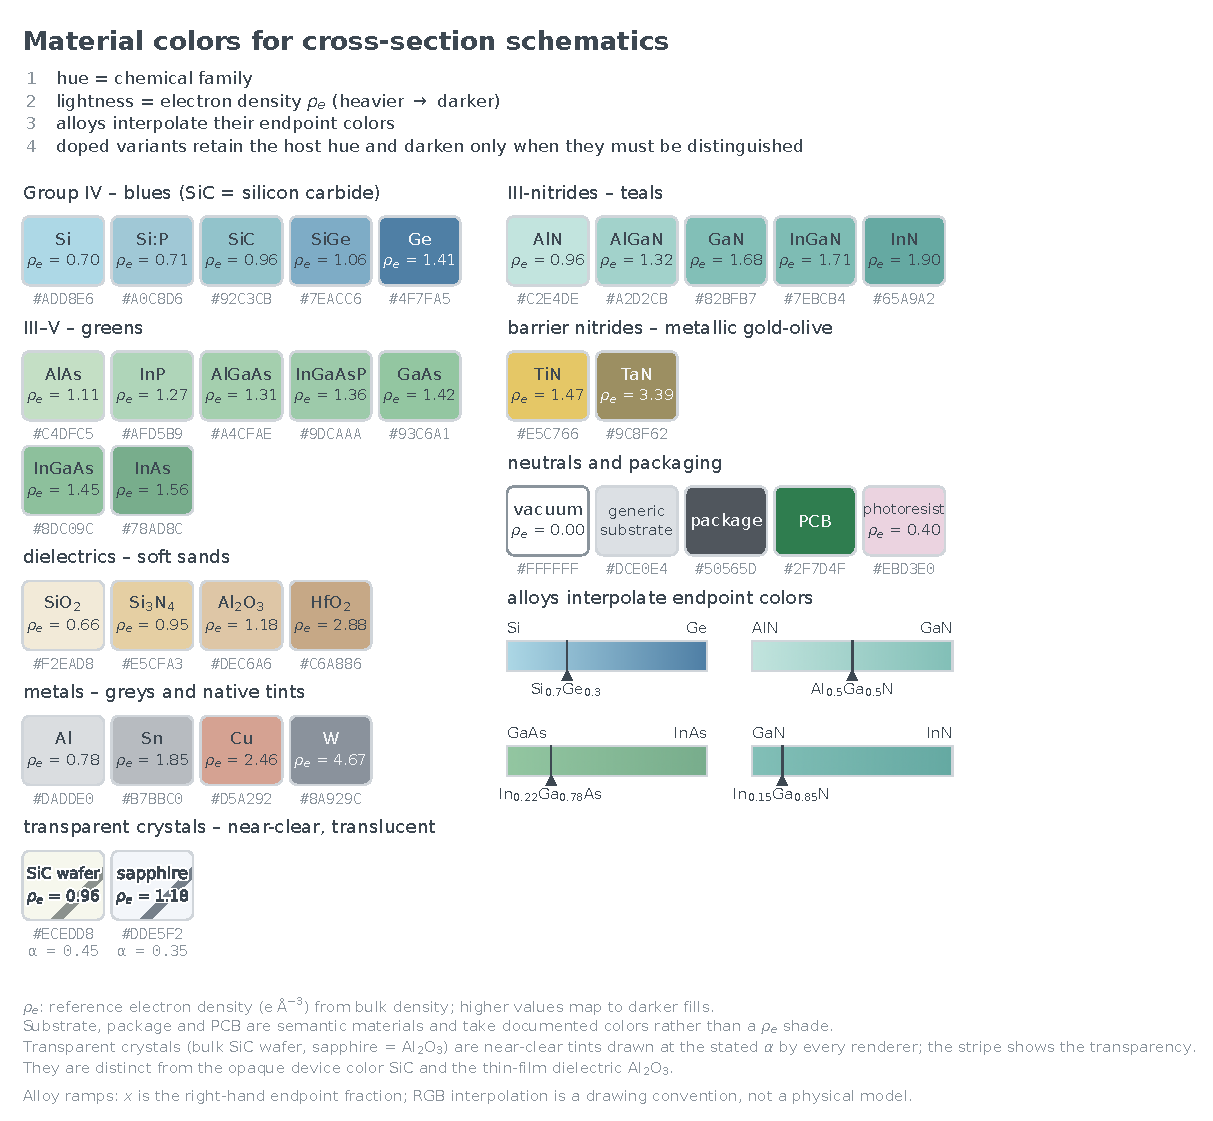
\includegraphics[width=0.98\textwidth,height=0.67\textheight,keepaspectratio]
    {material_palette.pdf}
  \caption{\kindspecial The semiconductor material palette: physical families on the left,
  nitrides, barriers, packaging materials and alloy ramps on the right, all on
  one chip grid. The last row on the left holds the transparent crystals, a
  bulk SiC wafer and sapphire (Al$_2$O$_3$). These are near-clear tints that
  every renderer draws at the stated alpha (the stripe behind each chip shows the
  transparency). They are distinct from the opaque device color SiC and
  the thin-film dielectric Al$_2$O$_3$.
  \generatedwith{examples/fig\_material\_palette.py}.}
\end{figure}

\clearpage
\section{Cross-sections and stack galleries}

Layered structures are the simplest use case. The drawing code handles
material lookup, alloy colors, repeated stacks, thickness annotations and
consistent labeling, which leaves the geometry free to stay deliberately
schematic. Six stacks that recur in metrology work are collected below, from
a high-k metal gate to a W/Si multilayer mirror.

\begin{figure}[H]
  \centering
  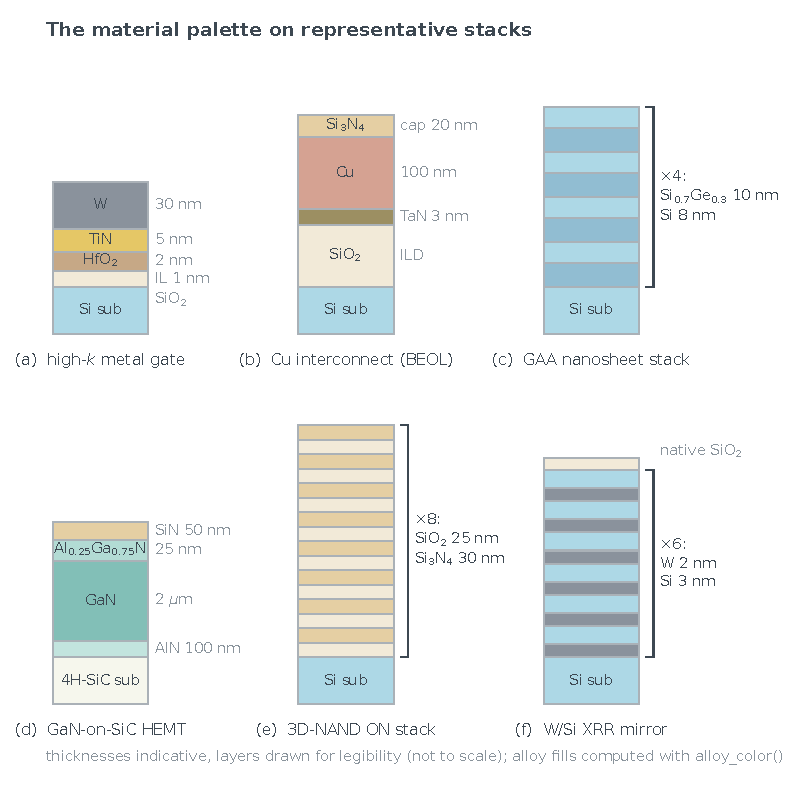
\includegraphics[width=0.98\textwidth,height=0.58\textheight,keepaspectratio]
    {stack_gallery.pdf}
  \caption{\kindspecial Representative metrology structures.
  \generatedwith{examples/fig\_stack\_gallery.py}.}
\end{figure}

\clearpage
\section{The transistor line-up in two renderings}

One geometry, drawn twice, separates what the package fixes from what the
author chooses. Both figures below are special-purpose compositions: their
scripts place solids directly rather than running a fabrication sequence,
because a line-up of four devices at one scale is a layout problem and not a
process. Parallel projection preserves the technical-diagram look, and
transparency exposes the channels inside a wrap-around gate.

Only the 3D panels are rasterized. Everything else in the saved PDF,
including the labels, the leaders and the cross-sections, stays vector, so
the page can be enlarged without softening the text.

The second rendering answers a request that comes up often. An author who
needs the colors of a familiar diagram can have them, and the role scheme is
then a deliberate exception to the palette law, written in a separate script
so the material-colored figures stay the default.

\begin{figure}[H]
  \centering
  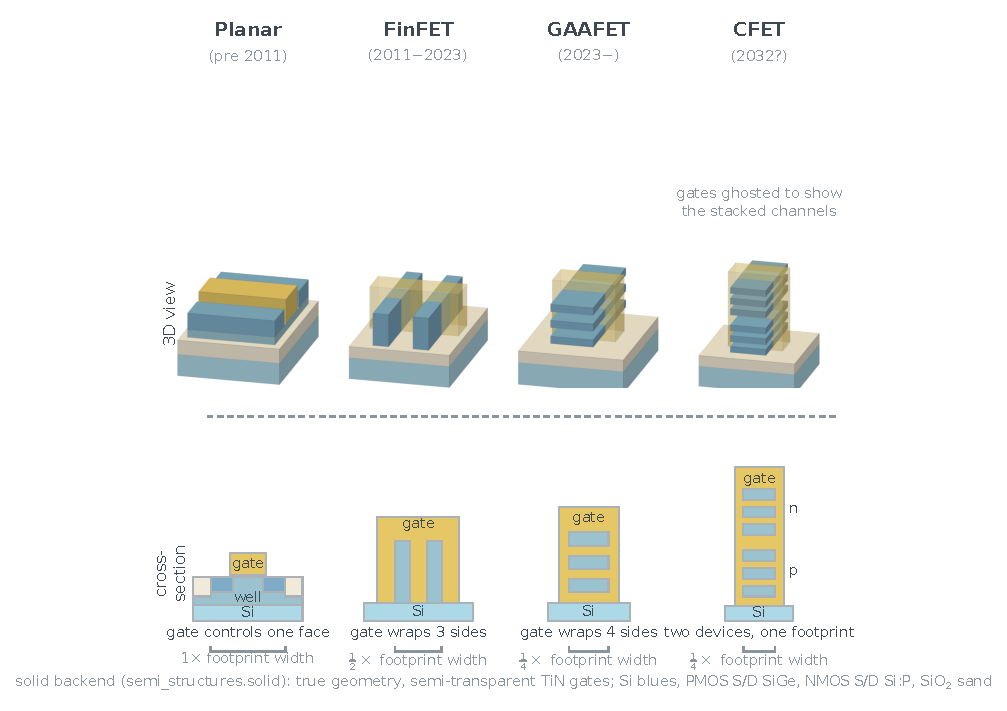
\includegraphics[width=0.96\textwidth,height=0.58\textheight,keepaspectratio]
    {transistor_evolution_solid.pdf}
  \caption{\kindspecial The transistor sequence rebuilt with
  \packagefile{semi\_structures.solid}. The PDF combines rasterized 3D panels
  with vector labels and cross-sections. The planar section is cut along the
  channel rather than across it, because the across-channel cut of a planar
  device shows only a stack of layers. Its active region still spans the
  footprint bracket, so the widths stay comparable.
  \generatedwith{examples/fig\_transistor\_solid.py}.}
\end{figure}

\begin{figure}[H]
  \centering
  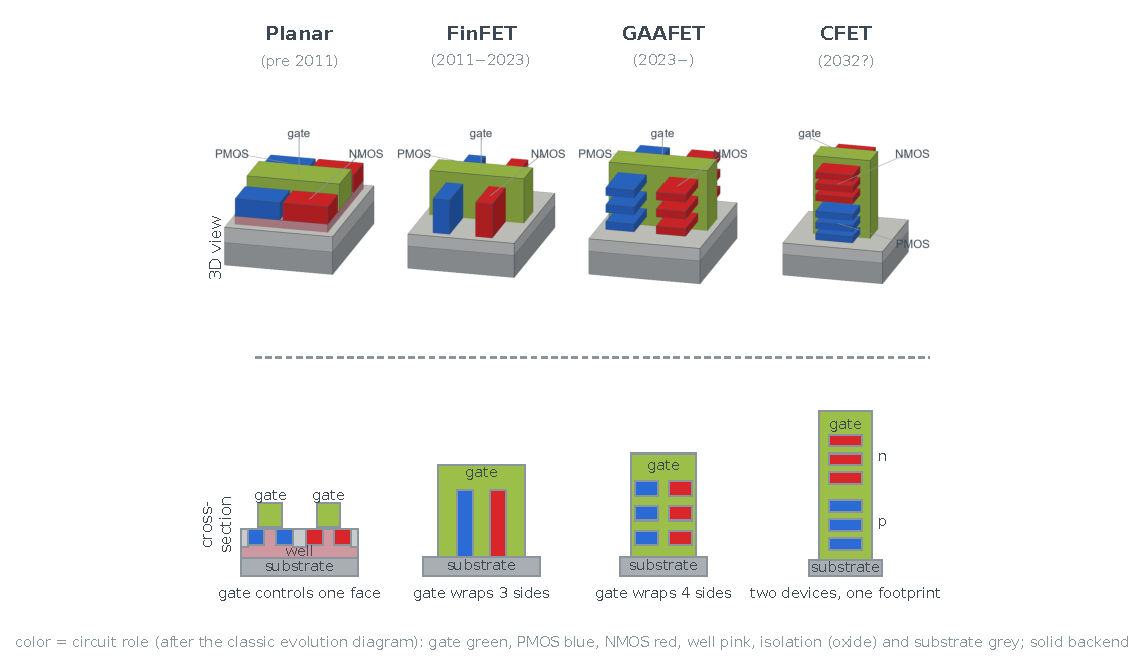
\includegraphics[width=0.96\textwidth,height=0.58\textheight,keepaspectratio]
    {transistor_evolution_rolecolor.pdf}
  \caption{\kindspecial The same four devices redrawn in the role colors of the
  classic evolution diagram (gate green, PMOS blue, NMOS red, well pink,
  isolation and substrate gray), with a PMOS/NMOS pair in every device,
  rendered as true solids on the solid backend so fins and nanosheets emerge
  from opaque gates. The planar section is cut along the channel, which is
  the only cut that shows a source, a drain and a gate over the channel
  between them. Color here means circuit role, not material.
  \generatedwith{examples/fig\_transistor\_evolution\_rolecolor.py}.}
\end{figure}


\clearpage
\section{Substrates and orientation features}

Every flow in this document starts from a substrate. A circular wafer is a
true cylinder rather than a disc drawn to look like one, and its orientation
feature is Boolean-cut from the solid, so the notch survives a cutaway and
appears correctly in a cross-section.

The cut also reaches every film that inherits the wafer footprint, which is
what a blanket deposition does by default. A film given its own footprint is
left alone, because it does not extend to the wafer edge. Nothing is
deposited in the two panels below, so they show the starting point on its
own.

\begin{figure}[H]
  \centering
  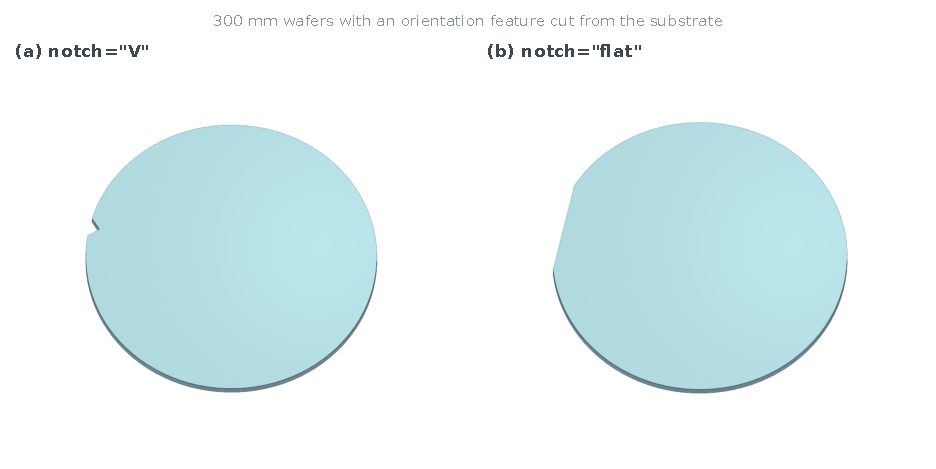
\includegraphics[width=0.98\textwidth,height=0.42\textheight,keepaspectratio]
    {wafer_notch.pdf}
  \caption{\kinddsl Bare 300 mm substrates carrying only their orientation
  feature: \packagefile{Wafer(size=300*mm, shape="circle", notch="V")} cuts a
  90$^\circ$ V-notch and \packagefile{notch="flat"} cuts a major flat.
  \packagefile{notch\_angle} places the feature and
  \packagefile{notch\_depth} or \packagefile{flat\_length} sizes it, with
  defaults exaggerated for legibility. The substrate thickness is exaggerated
  too, because a 775 $\mu$m wafer is invisibly thin beside a 300 mm diameter.
  \generatedwith{examples/fig\_wafer\_notch.py}.}
\end{figure}

\clearpage
\section{Special-purpose figures}

Not every useful figure is a process. Film stress bends a wafer, which no
flat cross-section can show, so the bow is applied to the slabs themselves
and the films are bent with it.

\begin{figure}[H]
  \centering
  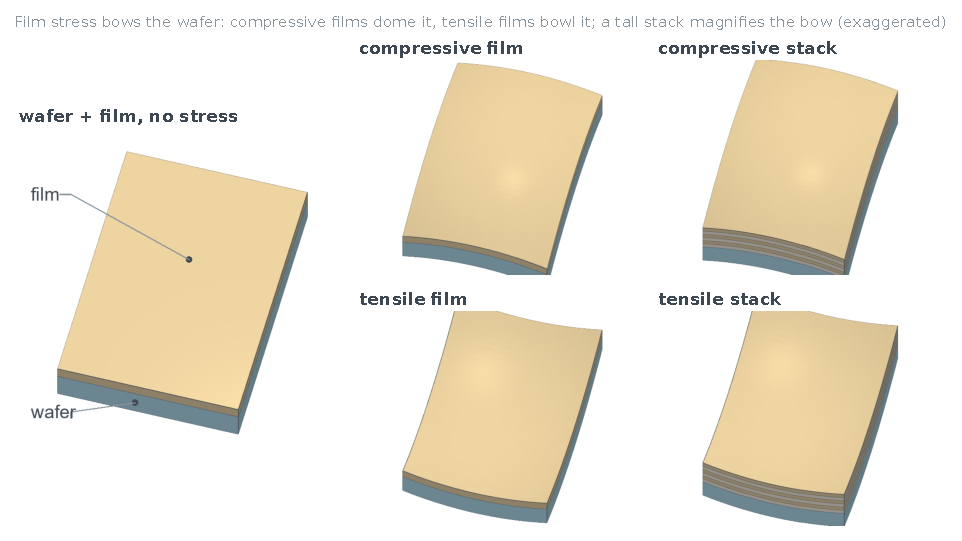
\includegraphics[width=0.98\textwidth,height=0.40\textheight,keepaspectratio]
    {film_stress_bow.pdf}
  \caption{\kindspecial Film stress bows the wafer. A flat wafer with one film gives the reference. A
  compressive film domes the pair and a tensile film bowls it, and a
  multilayer (an ON stack) magnifies the bow. \packagefile{Scene.box(..., bow=(sx, sy))} bends every
  slab with the same displacement, so films stay conformal. Bows are
  exaggerated and callouts are stick-and-ball (\packagefile{marker="dot"}).
  \generatedwith{examples/fig\_film\_stress\_bow.py}.}
\end{figure}

\clearpage
\section{The process language in use}

A structure written as a fabrication sequence reads like a run sheet, and the
renderer follows from the geometry rather than from a decision taken in
advance. This section works through that language in order, from the
individual verbs to a finished flow written to a file.

The same structure can be specified as a readable fabrication sequence. Six
snapshots expose substrate construction, blanket and repeated deposition,
depth-controlled rectangle, circle and rotated-ellipse etches, exact-shape
fill with optional overfill, and a patterned top layer. The three openings
share one line at a constant pitch and the top layer is a 1D grating of equal
lines, so the panels show a deliberate layout rather than scattered test
shapes.

\begin{figure}[H]
  \centering
  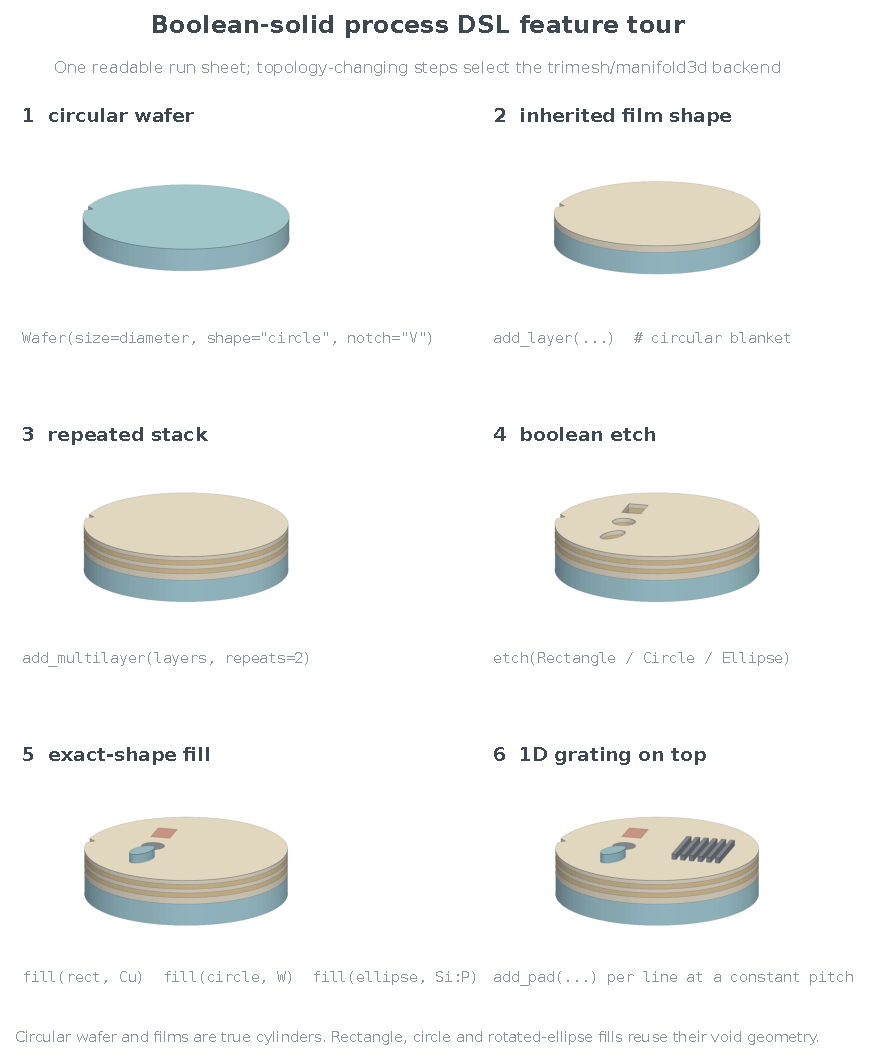
\includegraphics[width=0.86\textwidth,height=0.66\textheight,keepaspectratio]
    {dsl_feature_tour.pdf}
  \caption{\kinddsl A process-DSL regression example rendered with
  trimesh/manifold3d booleans and PyVista. Each panel is one circular
  \packagefile{Wafer} state. The three etched openings keep genuinely
  different geometries while sharing one line, and their fills reuse the void
  shapes exactly. Step 6 adds a 1D grating of six equal lines at a constant
  pitch, which is what a patterned top layer usually is.
  \generatedwith{examples/fig\_dsl\_feature\_tour.py}.}
\end{figure}

Shapes are shared between operations rather than restated. One
\packagefile{Rectangle}, \packagefile{Circle} or \packagefile{Ellipse}
object can drive a film footprint, an etch and the fill that lands in it, so
a rotated opening and its contents cannot drift apart. The planar prefix of
such a flow is eligible for the vector renderer on a rectangular die, while a
full-wafer example selects the solid backend immediately, because its
substrate and every inherited film are circular cylinders.

\begin{figure}[H]
  \centering
  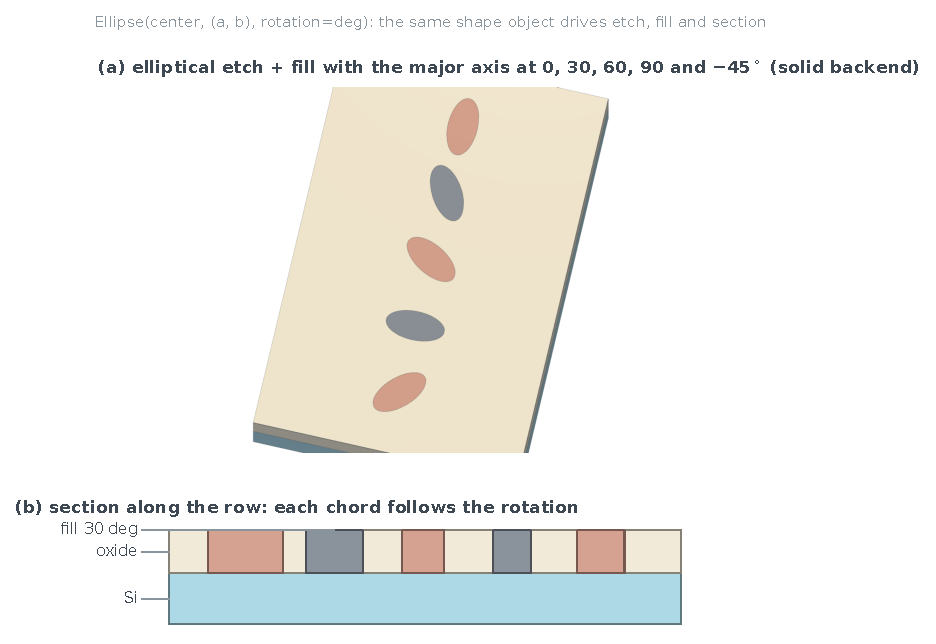
\includegraphics[width=0.90\textwidth,height=0.50\textheight,keepaspectratio]
    {rotated_ellipses.pdf}
  \caption{\kinddsl Rotated shapes: five elliptical openings etched to the Si with the
  major axis at 0, 30, 60, 90 and $-45^\circ$
  (\packagefile{Ellipse(center, (a, b), rotation=deg)}) and filled with Cu and
  W. One shape object drives the exact rotated prisms of the solid backend
  (a) and the chords of the 2D section along the row (b).
  \generatedwith{examples/fig\_rotated\_ellipses.py}.}
\end{figure}

\clearpage
Nesting those two verbs produces the structures that motivated them. A
circular etch opens the deposited word-line stack, and progressively smaller
etch and fill pairs then form blocking oxide, charge-trap nitride, tunnel
oxide, poly-Si channel and oxide core as non-overlapping Boolean solids.

Because every shell is a real solid, the model can be cut open. The cutaway
subtracts a camera-facing corner from each part separately, so the exposed
faces are capped in their own material colors and the concentric fills read
in section. The planes sit on the last hole column before the oxide slit,
since a cut at the slit itself would present a blank wall.

\begin{figure}[H]
  \centering
  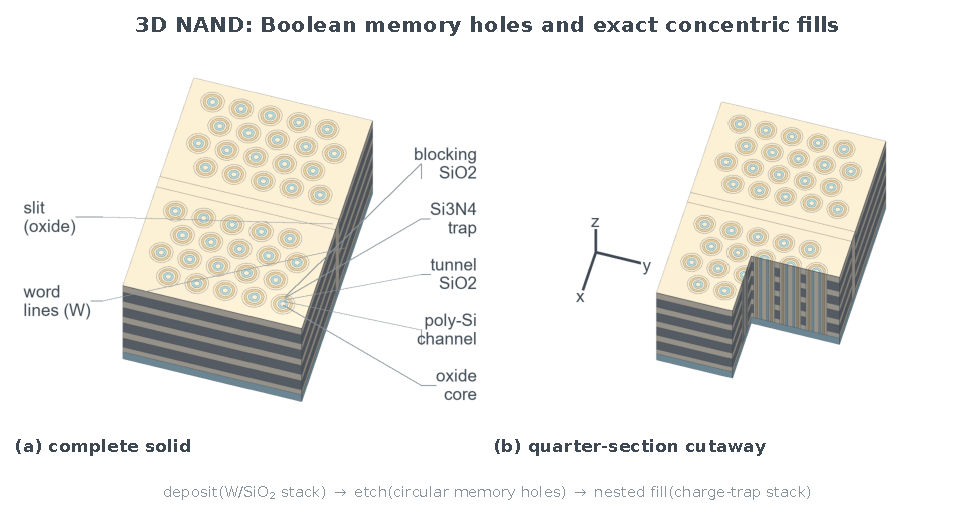
\includegraphics[width=0.99\textwidth,height=0.52\textheight,keepaspectratio]
    {nand3d.pdf}
  \caption{\kinddsl A process-DSL 3D-NAND diagram rendered with the Boolean solid
  backend: a hexagonal (close-packed) memory-hole array in two blocks
  separated by an oxide-filled slit, as in plan-view micrographs of real
  3D NAND, with nested concentric charge-trap fills in every hole
  (\packagefile{hex\_lattice()} supplies the centers). Panel (b) cuts the
  same model open at the same size and carries a labelled triad from
  \packagefile{Scene.axes()}. Two-line callouts keep the two panels equal.
  \generatedwith{examples/fig\_nand3d.py}.}
\end{figure}

\clearpage
Real stacks are taller than a page. A hundred repeated pairs can be deposited
and then drawn as the bottom ten and the top five, with everything that
crosses the elided interval cut there by every renderer, so the elision is a
property of the model rather than a trick played on one picture.

\begin{figure}[H]
  \centering
  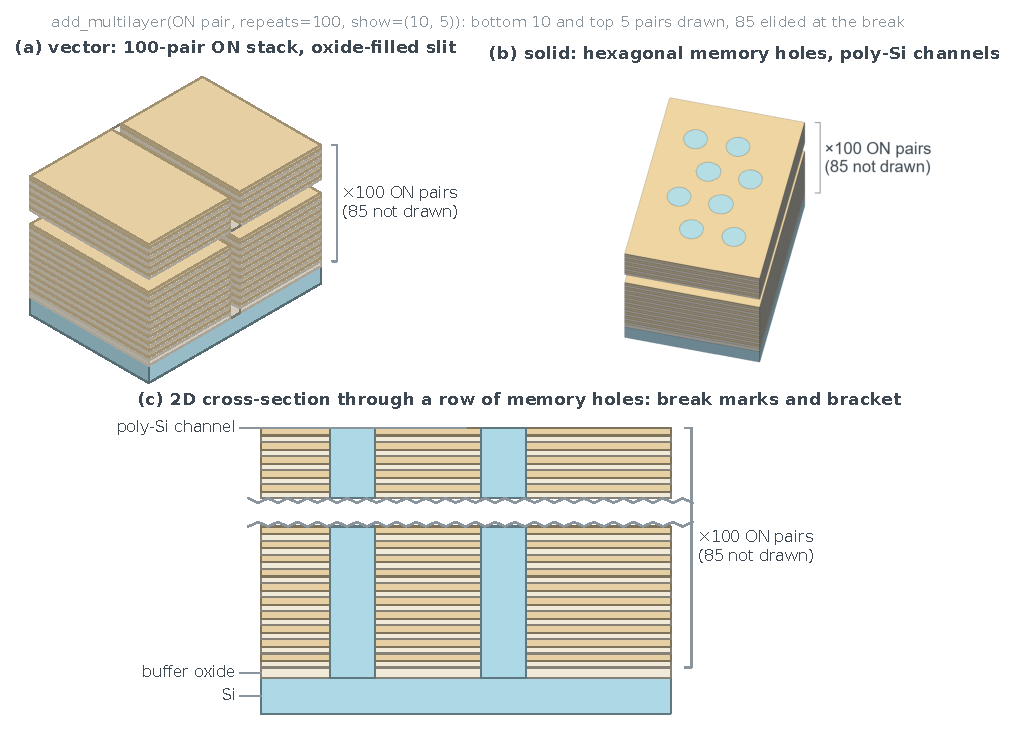
\includegraphics[width=0.98\textwidth,height=0.58\textheight,keepaspectratio]
    {nand_stack_break.pdf}
  \caption{\kinddsl Tall repeats without the clutter: a 100-pair SiO$_2$/Si$_3$N$_4$
  stack on Si drawn as its bottom ten and top five pairs with a stack break
  (\packagefile{add\_multilayer(..., repeats=100, show=(10, 5))}). Everything
  crossing the break is cut there by both 3D renderers. That includes the
  films, the oxide-filled slit in (a) and the hexagonal memory holes and
  channels in (b),
  and (c) is the 2D cross-section of the same model from the new section
  renderer (\packagefile{render(view="section")}), with zigzag break marks.
  every panel brackets the block ``$\times$100 ON pairs (85 not drawn)''.
  \generatedwith{examples/fig\_nand\_stack\_break.py}.}
\end{figure}

\clearpage
A flow is not always a single picture. The same model can be captured after
each step and drawn as a row of cross-sections, which is how a process is
usually explained on a slide or in a lecture.

\begin{figure}[H]
  \centering
  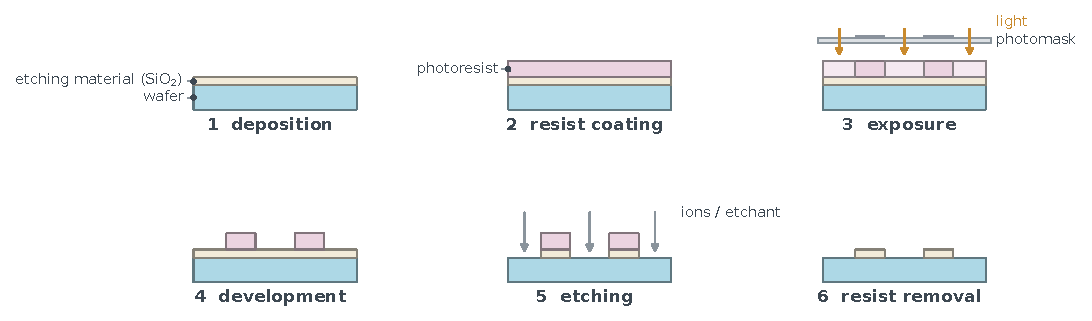
\includegraphics[width=0.98\textwidth,height=0.34\textheight,keepaspectratio]
    {litho_flow.pdf}
  \caption{\kinddsl A process flow as a sequence of sections: photolithography in six
  \packagefile{Wafer} states drawn by the 2D section renderer. The steps are
  deposition, resist coating, exposure through a photomask, development and
  film etch as rectangular etches through the same openings and resist
  removal with the \packagefile{strip()} verb. Exposure is a material
  replacement in the resist. The mask, the light and the ions are
  annotations, and the light uses the reserved beam color.
  Callouts are stick-and-ball.
  \generatedwith{examples/fig\_litho\_flow.py}.}
\end{figure}

The same six states can be drawn as solids instead. A section says what the
layers are, while the 3D view says what the pattern is, and in this case it
shows that the openings are trenches running the width of the die rather than
isolated holes.

\begin{figure}[H]
  \centering
  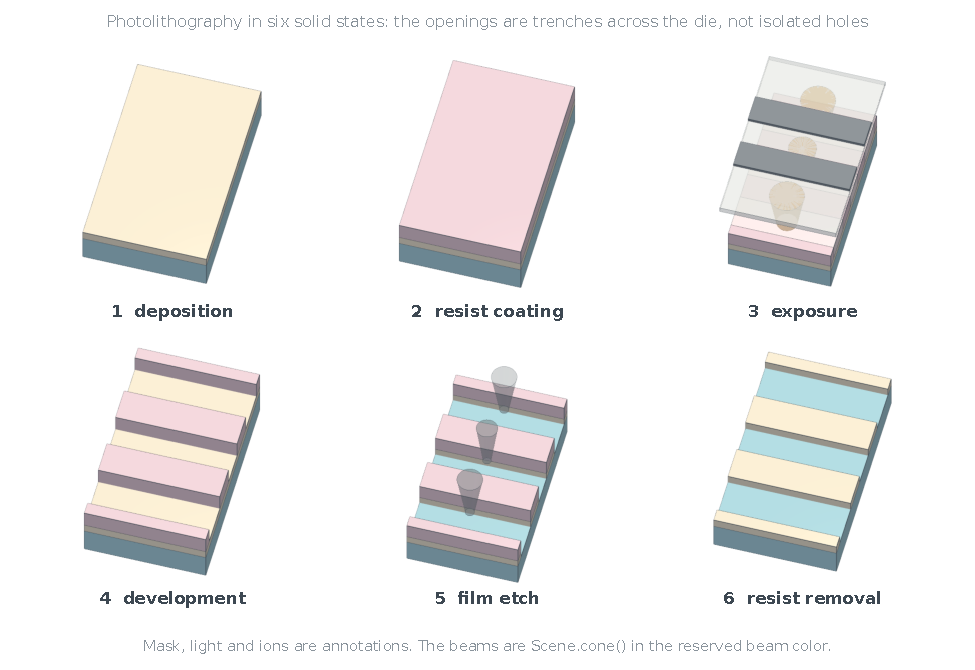
\includegraphics[width=0.81\textwidth,height=0.47\textheight,keepaspectratio]
    {litho_flow_3d.pdf}
  \caption{\kinddsl The photolithography flow of the previous figure rendered
  by the solid backend, one panel per \packagefile{Wafer} state. The
  photomask, the exposure light and the ions are annotations rather than
  process steps, and the beams are tapered \packagefile{Scene.cone()} solids
  in the reserved beam color.
  \generatedwith{examples/fig\_litho\_flow\_3d.py}.}
\end{figure}

Finally, a model can be written down. The document records the ordered calls
rather than the geometry they produce, which keeps it short enough to read
and exact enough to replay.

\begin{figure}[H]
  \centering
  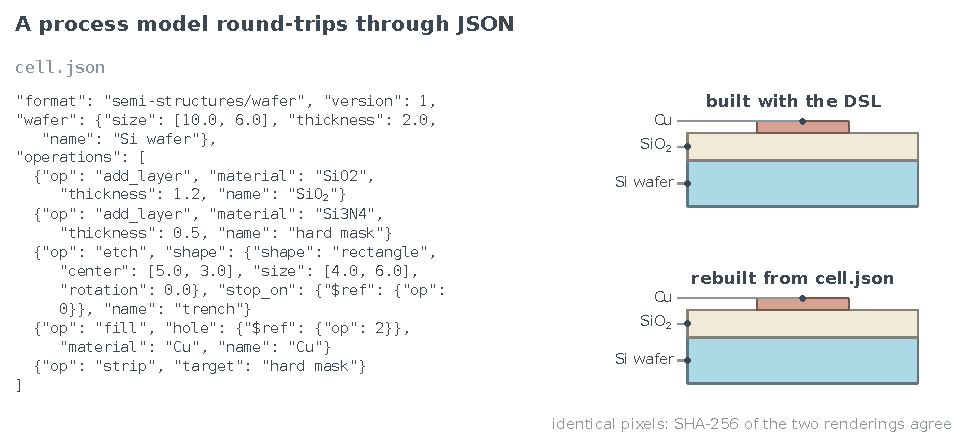
\includegraphics[width=0.98\textwidth,height=0.42\textheight,keepaspectratio]
    {serialization_roundtrip.pdf}
  \caption{\kinddsl A process model saved as JSON and rebuilt from it. The document
  stores the \emph{recipe}, which is the ordered DSL calls with their
  arguments, rather than the derived geometry, so replaying it reconstructs every layer,
  hole and fill. Arguments left at their defaults are omitted, and feature
  references such as \packagefile{stop\_on} and \packagefile{fill} are stored
  as \packagefile{\$ref} addresses into the operation list, which makes them
  independent of naming. The two renderings are compared by SHA-256 of their
  pixels: the reproduced model is not merely similar but the same picture.
  \generatedwith{examples/fig\_serialization\_roundtrip.py}.}
\end{figure}

\clearpage
\section{Solid-backend labels tied to 3D features}

Callouts can now be authored directly on a solid scene. Each anchor is a 3D
feature coordinate that follows camera changes, while its label position and
optional elbow points use normalized screen coordinates for stable publication
layout. Leaders terminate at the text boundary and labels remain horizontal.
The supplied visual reference was traced to Hanwha's feature on HBM
packaging. The panel below is an independent schematic rather than a
reproduction of that image.\ \cite{HanwhaHBM}

\begin{figure}[H]
  \centering
  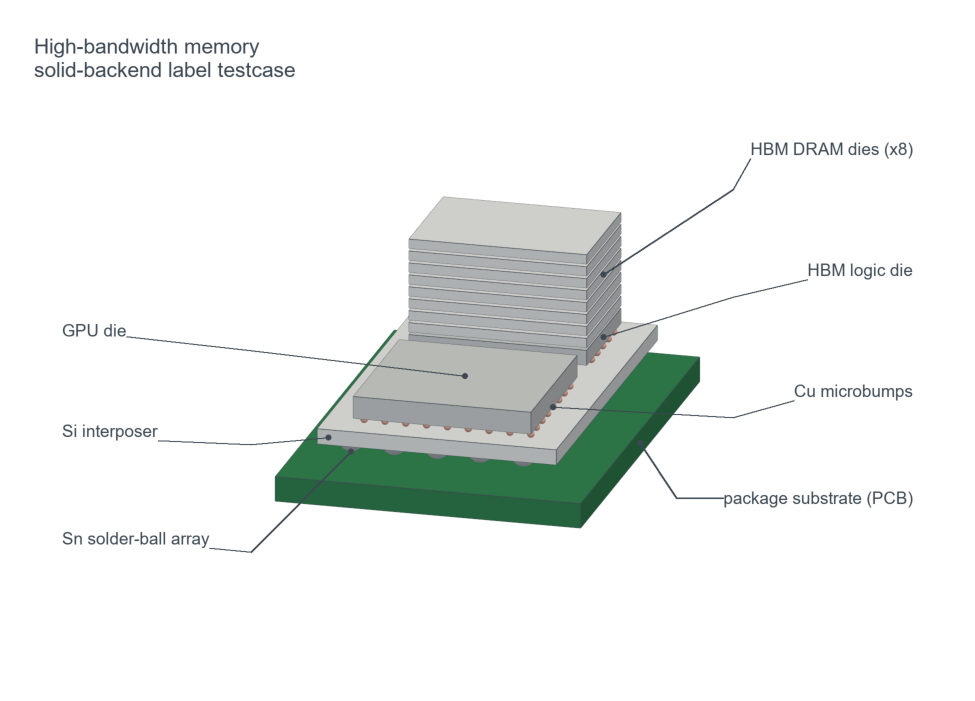
\includegraphics[width=0.98\textwidth,height=0.58\textheight,keepaspectratio]
    {hbm_labeled.pdf}
  \caption{\kindspecial An HBM package testcase. The solid backend creates the PCB
  package substrate, interposer, GPU, eight-die HBM stack, microbumps and Sn
  solder-ball array. In this packaging view the silicon parts take the
  neutral die gray (logic dies one shade darker) so the package materials
  carry the color. \packagefile{Scene.label()} supplies every routed
  callout, sized in points at print width.
  \generatedwith{examples/fig\_hbm\_labeled.py}.}
\end{figure}

\clearpage
\section{Miscellaneous structures}

Three device families that share no process but do share the drawing language: compound-semiconductor emitters, wide-bandgap power devices and a backside power-delivery block.

\subsection{III-V and III-nitride emitters}

Alloy-aware layer colors make it possible to compare six landmarks in one
drawing language. The sequence runs from the GaAs junction laser through the
double heterostructure, the DFB and surface-emitting cavities, the InGaN blue
LED and a mesa micro-LED. Each alloy fill is interpolated from its endpoint
materials, so an AlGaAs cladding sits visibly between AlAs and GaAs rather
than taking an arbitrary green.\ \cite{Hall1962,Hayashi1970,Kogelnik1971,Soda1979,Nakamura1994,Jiang2001}

\begin{figure}[H]
  \centering
  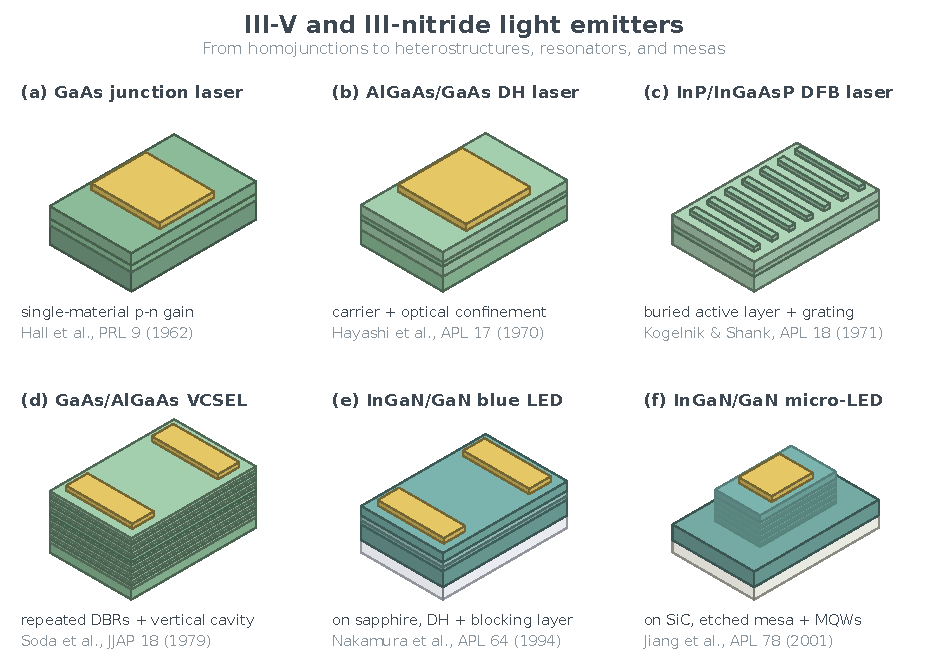
\includegraphics[width=0.89\textwidth,height=0.50\textheight,keepaspectratio]
    {optoelectronic_devices.pdf}
  \caption{\kinddsl III-V laser and III-nitride LED structures. The micro-LED mesa is
  a field etch expressed through the process DSL. Because it is rectilinear
  the vector backend draws it exactly, in the same style as its neighbors.
  The two nitride emitters sit on transparent substrates, sapphire in (e) and
  a bulk SiC wafer in (f), drawn translucent by the palette's alpha.
  Dimensions are schematic and selected for visual comparison.
  \generatedwith{examples/fig\_optoelectronic\_devices.py}.}
\end{figure}

\clearpage
\subsection{4H-SiC power devices}

The power-device page exercises doped shades, vertical drift regions,
implanted wells, surface and trench gates, shielding regions and repeated fin
channels. Four structures are drawn: a Schottky diode with backside metal, a
planar DMOS, a trench MOSFET with nested oxide and gate fills, and a vertical
tri-gate MOSFET. Implanted regions keep the SiC hue and move one shade
darker, so doping never reads as a different material.\ \cite{Cooper2002,Vathulya2000,Zhou2017,Ramamurthy2021}

\begin{figure}[H]
  \centering
  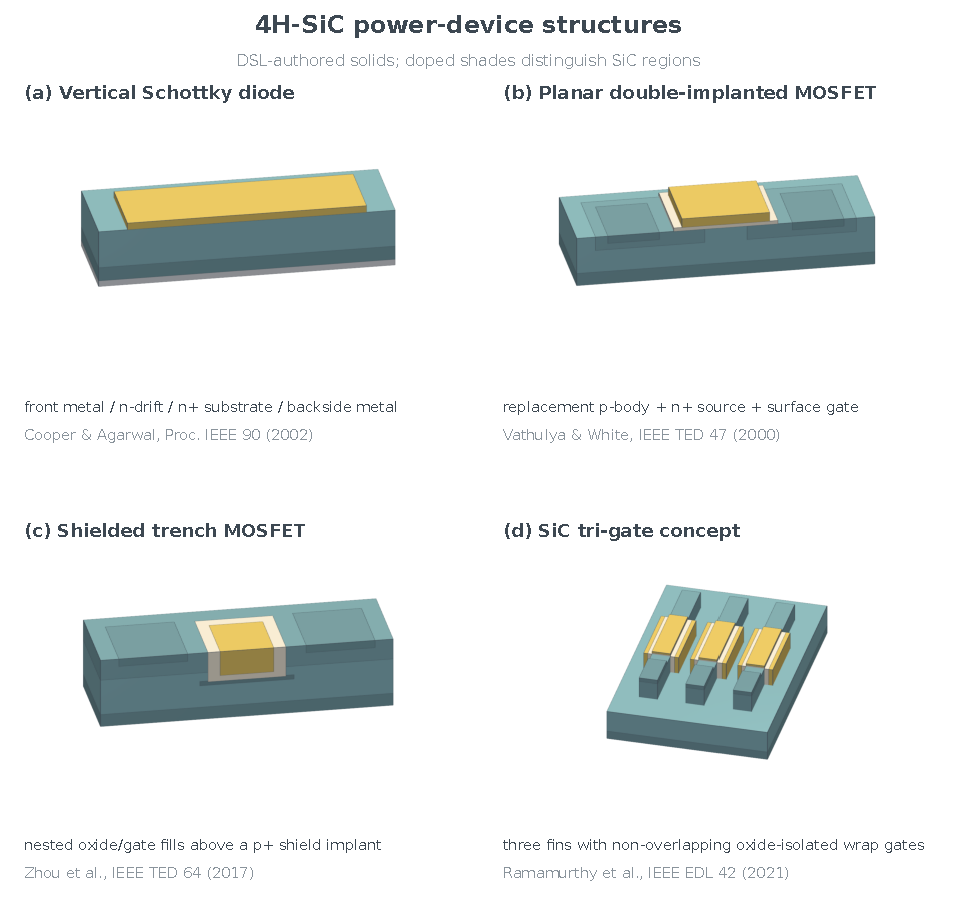
\includegraphics[width=0.88\textwidth,height=0.58\textheight,keepaspectratio]
    {sic_power_devices.pdf}
  \caption{\kinddsl Representative 4H-SiC power structures. Implants replace the drift
  material, and the trench oxide/gate are exact nested fills. Doped regions
  retain the SiC hue so material identity is not confused with circuit role.
  \generatedwith{examples/fig\_sic\_power\_devices.py}.}
\end{figure}

\clearpage
\subsection{Backside power delivery}

Backside power separates coarse power conductors from frontside signal
routing and connects them through nano-TSVs and buried rails. The geometry is
grounded in published buried-power-rail integrations.\ \cite{Prasad2019,Veloso2022VLSI,Veloso2022TED}
The two supplied visual references were traced to Intel's PowerVia Figure~4
and Aminext's nTSV explainer.\ \cite{IntelPowerVia,AminextBSP} The rendering
below is a new solid-model testcase, not a reproduction of either source.

\begin{figure}[H]
  \centering
  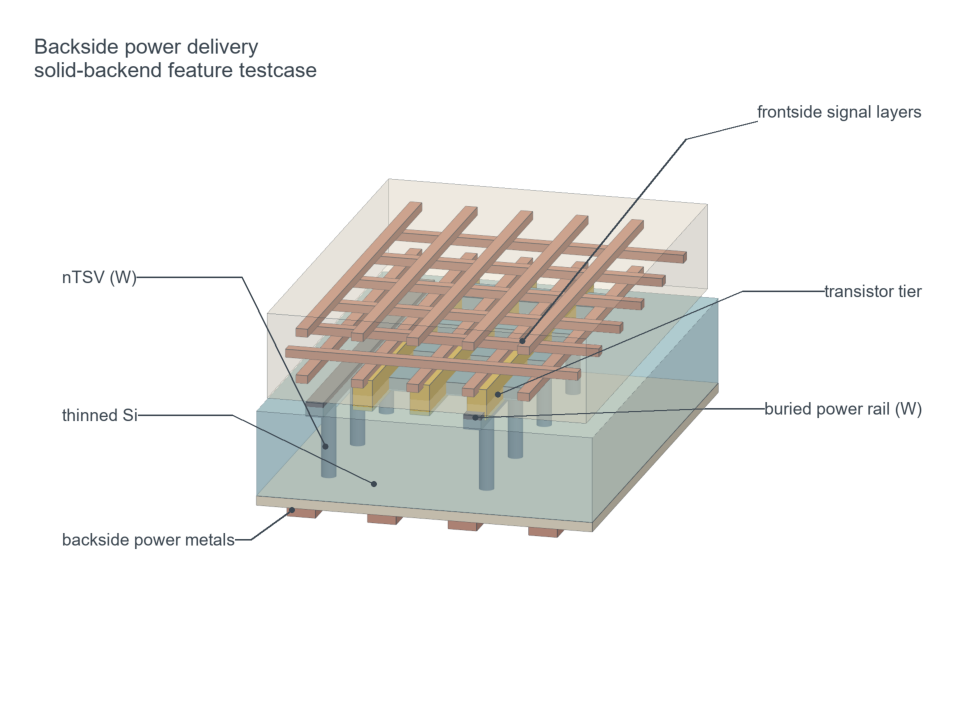
\includegraphics[width=0.98\textwidth,height=0.58\textheight,keepaspectratio]
    {backside_power_delivery.pdf}
  \caption{\kindspecial A labeled backside-power stack. Wide backside Cu, W nano-TSVs,
  buried W rails, a transistor tier and frontside Cu signal layers are
  separate true-solid objects. Each stick-and-ball callout was checked
  against the geometry and the rendered pixel, so every dot sits on a
  visible face of the part it names.
  \generatedwith{examples/fig\_backside\_power\_delivery.py}.}
\end{figure}

\begin{figure}[H]
  \centering
  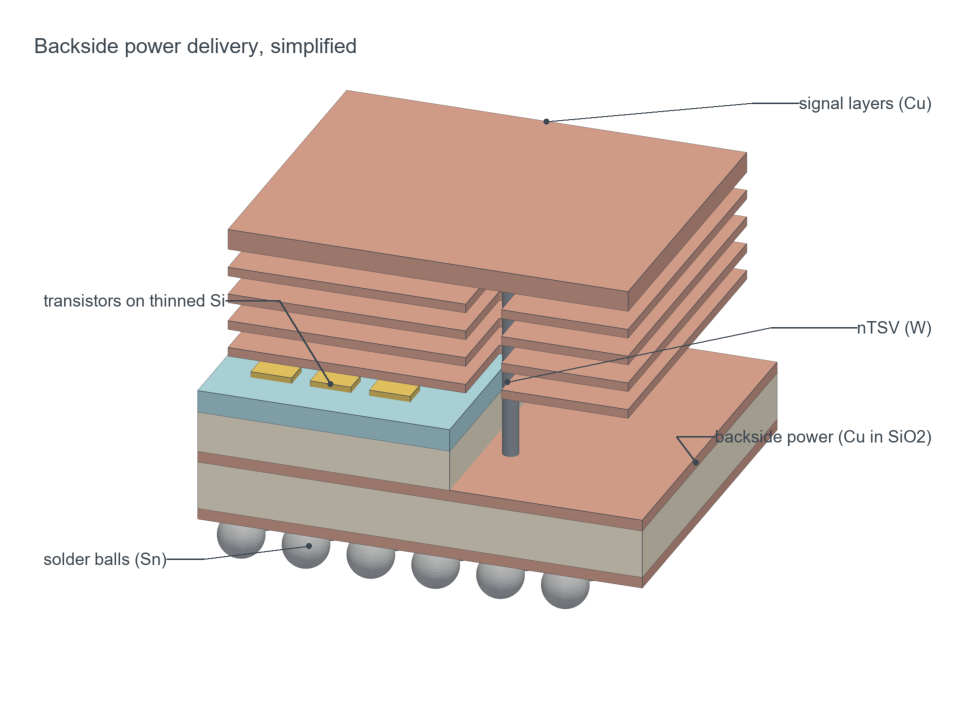
\includegraphics[width=0.90\textwidth,height=0.55\textheight,keepaspectratio]
    {backside_power_simple.pdf}
  \caption{\kindspecial The same idea as a simplified block, authored from a stylized
  reference illustration: Cu signal layers exploded above as plates, slotted
  where the single W nano-TSV runs up through them. Below that sit transistor
  pads on the thinned Si, a stepped backside power block of Cu sheets in
  SiO$_2$, and Sn solder balls. Color is material here. The reference's
  orange-on-dark scheme would be a presentation override.
  \generatedwith{examples/fig\_backside\_power\_simple.py}.}
\end{figure}


\clearpage
\section{Authoring from reference images}

The figures in this section were produced the way the introduction describes:
a multimodal coding assistant was given a reference image and asked to draw
the structure with the package. In each case the image supplied only the
composition, viewpoint and callout set. The geometry is new, schematic and
built from package primitives, and the reference images are not
redistributed (their provenance is recorded in
\packagefile{examples/REFERENCES.md}). The first two figures are the same
GPU package, assembled and then exploded, in the package's material palette.
The remaining two were requested \emph{in the colors of their
references}, as was the role-colored transistor line-up in Section 4. In each
case the override is the capability being demonstrated rather than an attempt
to reproduce the artwork, and deleting it returns the figure to the palette.
Circuit-role or presentation colors (raw hex fills, a dark
background) are permitted by both renderers, but they are deliberate
exceptions to the palette law and are kept as separate scripts so the
material-colored figures remain the defaults.

\begin{figure}[H]
  \centering
  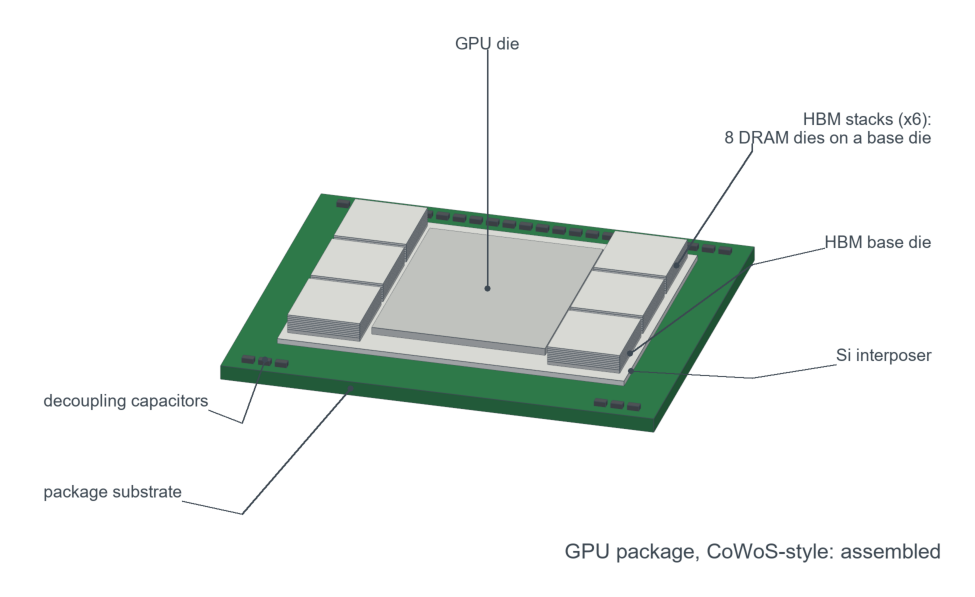
\includegraphics[width=0.98\textwidth,height=0.52\textheight,keepaspectratio]
    {gpu_cowos_assembled.pdf}
  \caption{\kindspecial A modern GPU package assembled, authored from a package
  photograph: the organic package substrate and its decoupling capacitors, the
  silicon interposer seated on its C4 bump field, and on top the GPU die
  flanked by six HBM towers, three per side. Assembled, both bump fields are
  hidden, so the callouts name only what the camera can see. Each is a
  stick-and-ball leader from \packagefile{Scene.label()}, and every anchor was
  checked against the geometry and the rendered pixel.
  \generatedwith{examples/fig\_gpu\_cowos\_assembled.py}.}
\end{figure}

\clearpage
\begin{figure}[H]
  \centering
  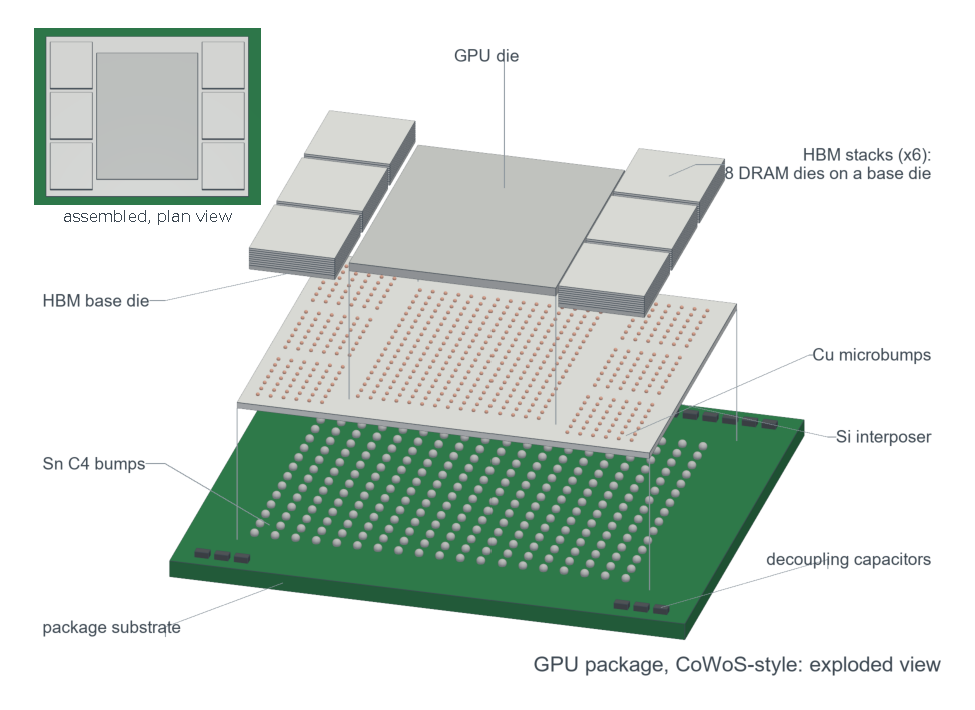
\includegraphics[width=0.98\textwidth,height=0.58\textheight,keepaspectratio]
    {gpu_cowos_exploded.pdf}
  \caption{\kindspecial A modern GPU package as an exploded chip-on-wafer-on-substrate
  (CoWoS-style) view, authored from a package photograph and a foundry
  exploded-view graphic: package substrate with its Sn C4 bump field and
  decoupling capacitors, Si interposer with Cu microbump fields under every
  die, and on top the GPU die flanked by six HBM towers (eight DRAM dies on
  a base die with Cu bond layers, three per side). Thin corner guide lines
  tie each level to the one below, and the inset repeats the previous
  figure from almost directly above, the plan view of the photograph.
  Silicon parts take the neutral die gray with the logic dies one shade
  darker, so PCB green, Sn and Cu carry the color.
  \generatedwith{examples/fig\_gpu\_cowos\_exploded.py}.}
\end{figure}

\clearpage
\begin{figure}[H]
  \centering
  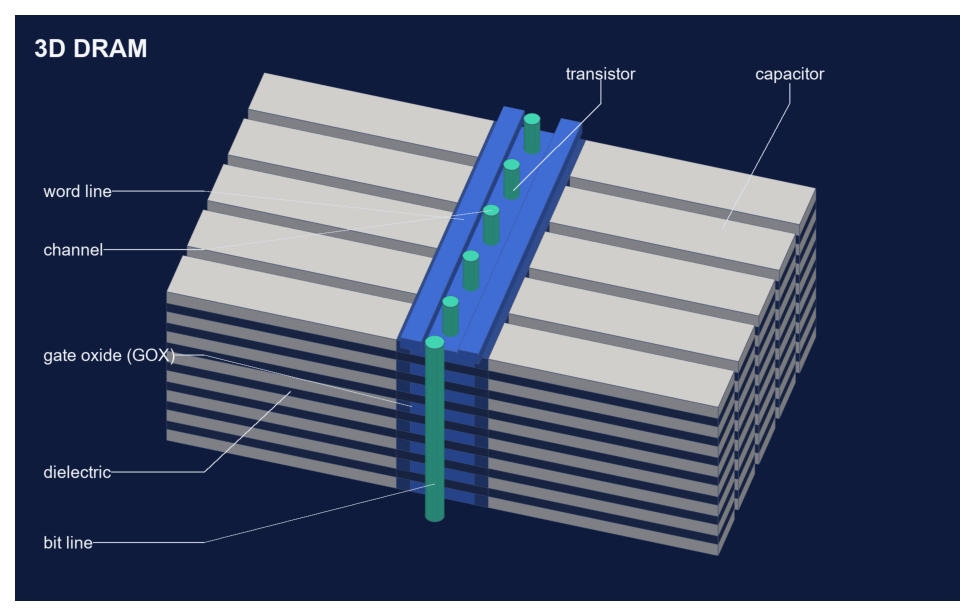
\includegraphics[width=0.98\textwidth,height=0.58\textheight,keepaspectratio]
    {dram3d_reference_colors.pdf}
  \caption{\kindspecial A horizontal-capacitor 3D DRAM archetype in a vendor-style
  presentation scheme (dark background, light-gray capacitor plates, dark
  dielectric, blue word lines and transistors, teal channels and bit line,
  light callouts) using \packagefile{render(background=..., edge\_color=...)}.
  \generatedwith{examples/fig\_dram3d\_reference\_colors.py}.}
\end{figure}

\begin{figure}[H]
  \centering
  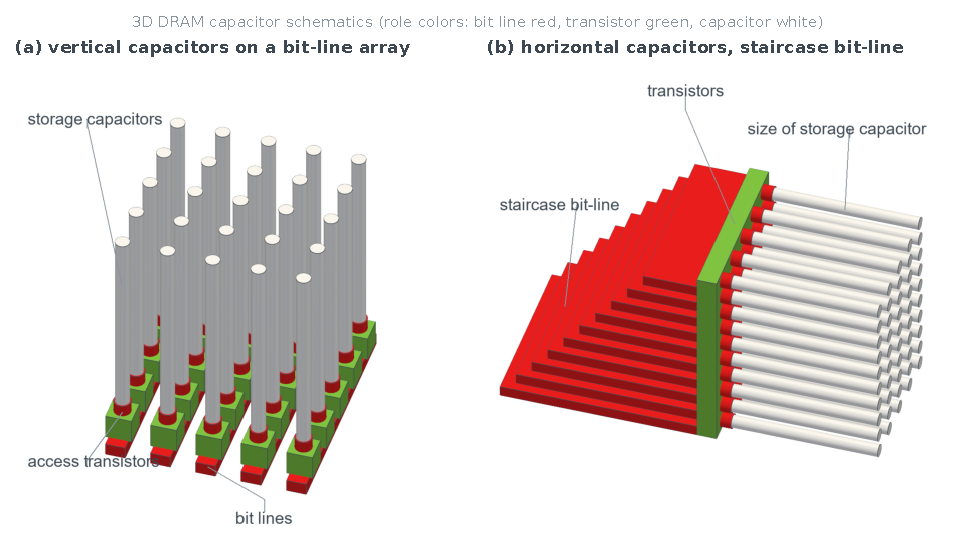
\includegraphics[width=0.98\textwidth,height=0.50\textheight,keepaspectratio]
    {dram3d_capacitor_schematics.pdf}
  \caption{\kindspecial Two 3D DRAM capacitor schematics in a red/green/white role scheme:
  (a) vertical storage capacitors on access transistors over a bit-line
  array. (b) Horizontal capacitors on a staircase bit-line, the capacitor
  length setting the storage size. Horizontal cylinders are rotated trimesh
  primitives added with \packagefile{Scene.add()}.
  \generatedwith{examples/fig\_dram3d\_capacitor\_schematics.py}.}
\end{figure}

\clearpage
\addcontentsline{toc}{section}{References}
\small
\begin{thebibliography}{99}
\setlength{\itemsep}{0.18em}
\setlength{\parskip}{0pt}

\bibitem{Hisamoto2000}
D. Hisamoto et al., ``FinFET---A self-aligned double-gate MOSFET scalable to
20 nm,'' \emph{IEEE Transactions on Electron Devices} 47, 2320--2325 (2000),
\href{https://doi.org/10.1109/16.887014}{doi:10.1109/16.887014}.

\bibitem{Loubet2017}
N. Loubet et al., ``Stacked nanosheet gate-all-around transistor to enable
scaling beyond FinFET,'' \emph{Symposium on VLSI Technology} (2017),
\href{https://doi.org/10.23919/VLSIT.2017.7998183}{doi:10.23919/VLSIT.2017.7998183}.

\bibitem{HanwhaHBM}
Hanwha, ``Powering AI: Advanced semiconductor manufacturing solutions,''
feature story (2024),
\href{https://www.hanwha.com/newsroom/news/feature-stories/powering-ai-semiconductor-manufacturing-solutions.do}{source page}.

\bibitem{Hall1962}
R. N. Hall et al., ``Coherent Light Emission From GaAs Junctions,''
\emph{Physical Review Letters} 9, 366 (1962),
\href{https://doi.org/10.1103/PhysRevLett.9.366}{doi:10.1103/PhysRevLett.9.366}.

\bibitem{Hayashi1970}
I. Hayashi et al., ``Junction Lasers Which Operate Continuously at Room
Temperature,'' \emph{Applied Physics Letters} 17, 109--111 (1970),
\href{https://doi.org/10.1063/1.1653326}{doi:10.1063/1.1653326}.

\bibitem{Kogelnik1971}
H. Kogelnik and C. V. Shank, ``Stimulated Emission in a Periodic Structure,''
\emph{Applied Physics Letters} 18, 152--154 (1971),
\href{https://doi.org/10.1063/1.1653605}{doi:10.1063/1.1653605}.

\bibitem{Soda1979}
H. Soda et al., ``GaInAsP/InP Surface Emitting Injection Lasers,''
\emph{Japanese Journal of Applied Physics} 18, 2329--2330 (1979),
\href{https://doi.org/10.1143/JJAP.18.2329}{doi:10.1143/JJAP.18.2329}.

\bibitem{Nakamura1994}
S. Nakamura, T. Mukai, and M. Senoh, ``Candela-class high-brightness
InGaN/AlGaN double-heterostructure blue-light-emitting diodes,''
\emph{Applied Physics Letters} 64, 1687--1689 (1994),
\href{https://doi.org/10.1063/1.111832}{doi:10.1063/1.111832}.

\bibitem{Jiang2001}
H. X. Jiang et al., ``III-nitride blue microdisplays,'' \emph{Applied Physics
Letters} 78, 1303--1305 (2001),
\href{https://doi.org/10.1063/1.1351521}{doi:10.1063/1.1351521}.

\bibitem{Cooper2002}
J. A. Cooper and A. Agarwal, ``SiC power-switching devices---the second
electronics revolution?'' \emph{Proceedings of the IEEE} 90, 956--968 (2002),
\href{https://doi.org/10.1109/JPROC.2002.1021561}{doi:10.1109/JPROC.2002.1021561}.

\bibitem{Vathulya2000}
V. R. Vathulya and M. H. White, ``Characterization of inversion and
accumulation layer electron transport in 4H- and 6H-SiC MOSFETs on implanted
p-type regions,'' \emph{IEEE Transactions on Electron Devices} 47,
2018--2023 (2000), \href{https://doi.org/10.1109/16.877161}{doi:10.1109/16.877161}.

\bibitem{Zhou2017}
X. Zhou et al., ``4H-SiC Trench MOSFET With Floating/Grounded Junction
Barrier-controlled Gate Structure,'' \emph{IEEE Transactions on Electron
Devices} 64, 4568--4574 (2017),
\href{https://doi.org/10.1109/TED.2017.2755721}{doi:10.1109/TED.2017.2755721}.

\bibitem{Ramamurthy2021}
R. P. Ramamurthy et al., ``The Tri-Gate MOSFET: A New Vertical Power
Transistor in 4H-SiC,'' \emph{IEEE Electron Device Letters} 42, 90--93 (2021),
\href{https://doi.org/10.1109/LED.2020.3040239}{doi:10.1109/LED.2020.3040239}.

\bibitem{Prasad2019}
D. Prasad et al., ``Buried Power Rails and Back-side Power Grids,''
\emph{IEEE International Electron Devices Meeting} (2019),
\href{https://doi.org/10.1109/IEDM19573.2019.8993617}{doi:10.1109/IEDM19573.2019.8993617}.

\bibitem{Veloso2022VLSI}
A. Veloso et al., ``Scaled FinFETs Connected by Using Both Wafer Sides for
Routing via Buried Power Rails,'' \emph{IEEE Symposium on VLSI Technology and
Circuits} (2022),
\href{https://doi.org/10.1109/VLSITechnologyandCir46769.2022.9830177}{doi:10.1109/VLSITechnologyandCir46769.2022.9830177}.

\bibitem{Veloso2022TED}
A. Veloso et al., ``Scaled FinFETs Connected by Using Both Wafer Sides for
Routing via Buried Power Rails,'' \emph{IEEE Transactions on Electron Devices}
69, 7173--7179 (2022), \href{https://doi.org/10.1109/TED.2022.3205561}{doi:10.1109/TED.2022.3205561}.

\bibitem{IntelPowerVia}
P. Ranade, M. Pant, S. Nimmagadda, and E. Fetzer, ``Cutting-edge Process
Technologies for Data Center,'' Intel Foundry, Figure 4,
\href{https://www.intel.com/content/www/us/en/foundry/library/advanced-process-technologies-for-data-center.html}{source page}.

\bibitem{AminextBSP}
Aminext, ``What is Backside Power Delivery (BSP)? Redefining the Chip Power
Map for the 2nm Revolution,'' nTSV diagram and process description (2025),
\href{https://www.aminext.blog/en/post/backside-power-delivery-bsp-explained-1}{source page}.

\end{thebibliography}
\normalsize

\end{document}
